% !TEX root = ../main.tex

\section{Firmware}
\label{sec:firmware}

\scaffold{
  \textbf{Paragraph 1, architecture} (about 90 words). The firmware is written in Rust \cite{rust2026} on the asynchronous Embassy framework \cite{embassy2026}, so measurement, USB and WiFi run as concurrent tasks \cite{benson2026expad}. One module knows the board, the drivers know chips, and the solver and the per-jack state machine form a separate library without hardware dependency. That library compiles for the host, where 52 tests drive the solver against a simulated star network and the state machine against a simulated jack in simulated time; they caught, for example, swapped high and low drives in the port from the simulator \cite{benson2026topologysim} before the code ever ran on hardware.
}

\scaffold{
  \textbf{Paragraph 2, jack monitor} (about 90 words, \cref{fig:firmware-overview}). One monitor per jack runs the stages of \cref{fig:firmware-overview}: rail measurement, plug detection, identification by solves, following, and the two ways back (identify again when the followed pedal no longer matches, plug detection when the plug is pulled). It never touches hardware: it hands out one reading at a time (drives and contact) and takes the voltage back, so a scheduler can interleave the jacks of both ADCs. The full state diagram is in \cref{fig:jack-monitor-states}.
}

\begin{figure}[htbp]
  \centering
  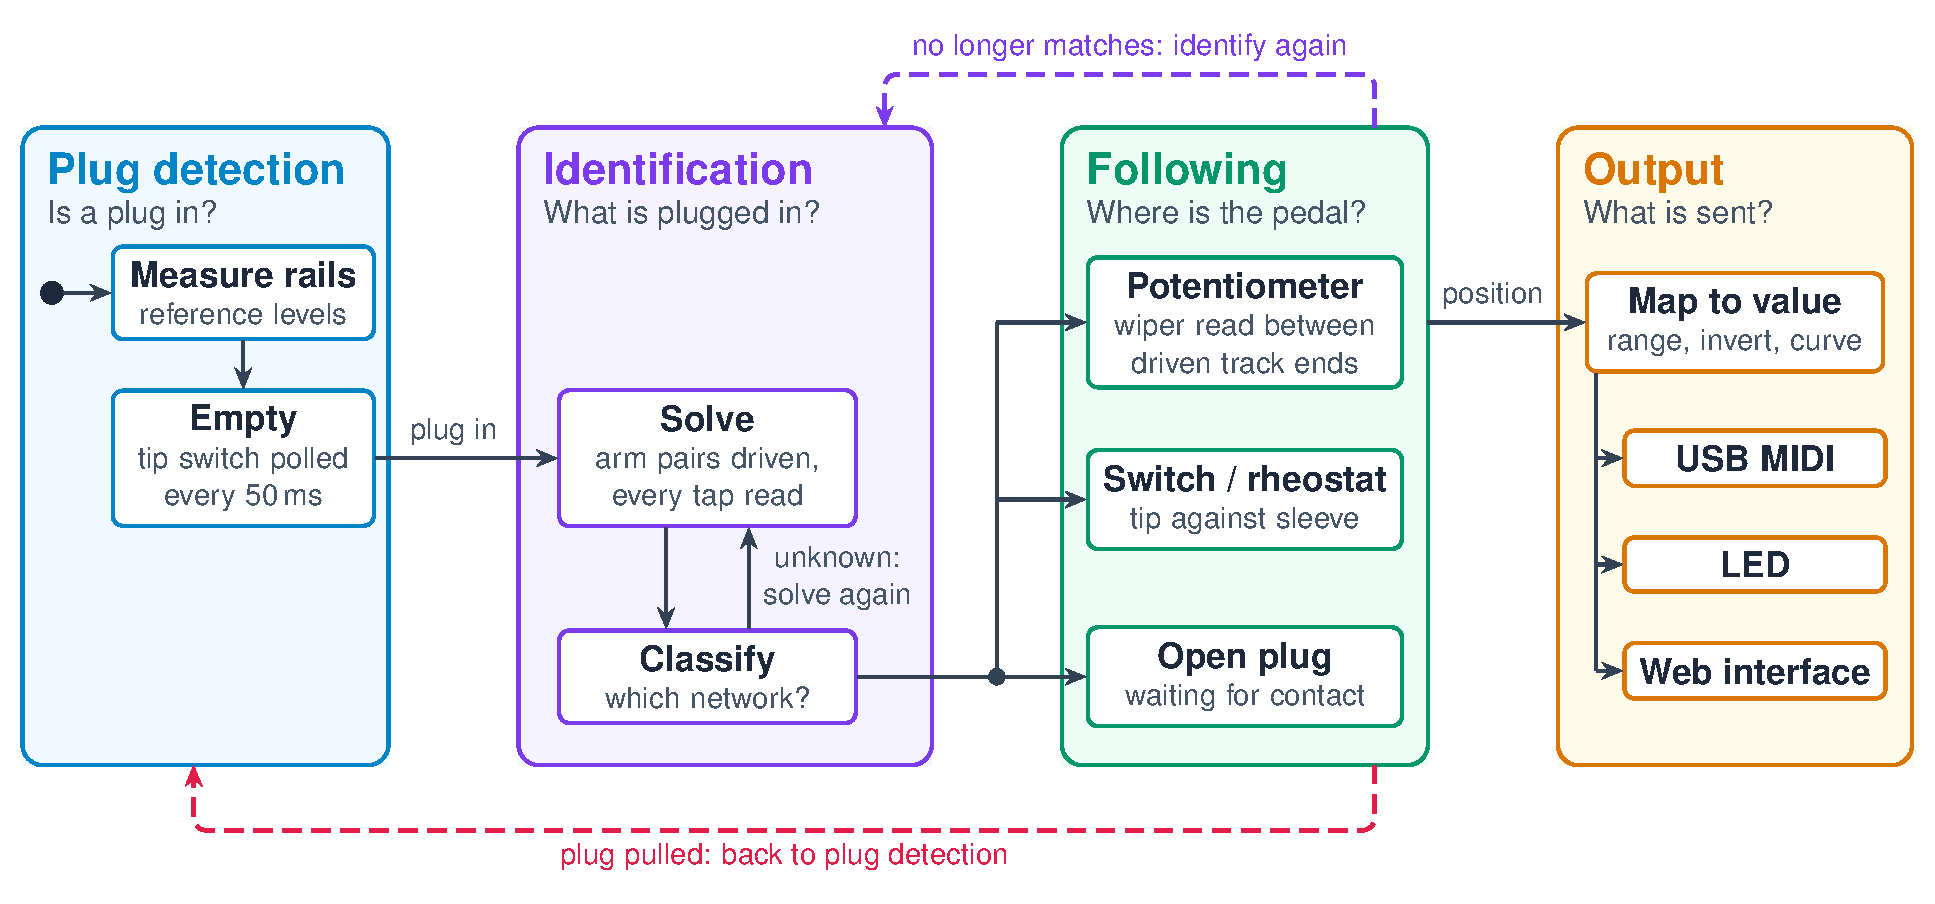
\includegraphics[width=0.85\linewidth]{04-implementation/figures/jack-monitor-overview}
  \titledcaption{Jack Monitor}{\scaffoldinline{The four stages per jack and the two ways back. Source: \code{docs/diagrams/jack-monitor-overview.tex}.}}
  \label{fig:firmware-overview}
\end{figure}

\scaffold{
  \textbf{Paragraph 3, update rate} (about 160 words). The target of 50 to \qty{100}{\hertz} came from the discussion after milestone~1; \qty{100}{\hertz} keeps the interval below the \qty{10}{\milli\second} commonly accepted as the bound of the audible reaction to a gesture \cite{wessel2002problems}. The first firmware solved every jack in turn: 382~ms per sweep, 2.6 updates per second. The diagnosis: every reading changed the ADC channel, and the sinc\textsuperscript{3} filter needs three conversion periods to settle after a change \cite{adi2001ad7718}, \qty{10.3}{\milli\second} at \qty{315}{\hertz}; four jacks times nine readings gave the sweep. Two steps fixed it. Reading faster: a characterization of all filter rates (\cref{tab:adc-characterization}) chose \qty{819}{\hertz}, 2.3 times faster at \qty{0.39}{\milli\volt} noise, which also exposed a poorly conditioned solve of the tip-wiper pedal and raised the minimum conditioning to 0.5. Reading less: an identified pedal is followed with one reading instead of re-solved, and empty jacks cost one plug check every \qty{50}{\milli\second}. Both ADCs convert in parallel, each serving its most overdue jack.
}

\scaffold{
  \textbf{Paragraph 4, output and web interface} (about 100 words). The position is stretched from the per-jack range to $[0, 1]$, inverted if set, and bent by a drive curve $y = (1+b)u/(1 - b + 2bu)$ with $b = 0.9\,d$ for a knob $d \in [-1, 1]$; this is Schlick's bias function \cite{schlick1994bias}, which keeps both ends fixed and gives the inverse curve for $-d$, so it straightens logarithmic and antilogarithmic pots alike. The device is a class-compliant USB MIDI device \cite{usbif1999midi} sending 7-bit control changes (controller 11 or 1 by default \cite{midi2026controlchange}), with a newer value replacing one not yet sent. A WiFi access point with a captive portal serves the web interface, which shows the identified network of each jack and holds the settings; they are not stored in flash yet.
}
